\documentclass{article} % For LaTeX2e
\usepackage{nips12submit_e,times}
%\documentstyle[nips12submit_09,times,art10]{article} % For LaTeX 2.09
\usepackage{amsmath,amsthm,amssymb, dsfont}
\usepackage{pgf}
\usepackage{tikz}
\def\I{\mathbb{I}}
\usetikzlibrary{arrows,automata}

\title{Infectious Knowledge in a Collaborative News Site}


\author{
Eliana Feasley\\
Department of Computer Science\\
University of Texas at Austin\\
\texttt{elie@cs.utexas.edu} \\
\And
Wesley Tansey\\
Department of Computer Science\\
University of Texas at Austin\\
\texttt{tansey@cs.utexas.edu} \\
}

\newcommand{\fix}{\marginpar{FIX}}
\newcommand{\new}{\marginpar{NEW}}
\def\c{\textbf{ Cite }}
\nipsfinalcopy

\begin{document}

\maketitle

\begin{abstract}
In recent years, the attention paid to cascading information in social networks has been increasing in a fashion itself comparable to a social cascade. This makes sense - the way that information infects different spaces of ideas has applications to basic graph theory, epidemiology, predictions of the future, and marketing. In this paper, we examine the dynamics of information spread across subcommunities with overlapping networks in several domains - the question-answering site \texttt{StackExchange}, a news network provided by memetracker, and a synthetic dataset of our own devising. Each of these is structured such that it is possible to track how ideas spread over time, and to discover semi-explicit communities and the connections between them.
\end{abstract}

\section{Introduction}
\label{intro}
Social cascades capture the concept of new ideas, or \textit{memes}, spreading across influence networks and infecting subcultures. Cascade theory has applications to several areas, including epidemiology, graph theory, machine learning, and marketing. In this project, we examine the dynamics of information spread across sub-communities with overlapping networks in several real-world domains: the social news site \textit{reddit}, a collection of blogs and mainstream media \cite{memetracker}, and the question-answer network \textit{StackExchange}. Our goal is to capture the flow of memes by learning a graphical model for each domain. We learn a graphical model describing the transition between timesteps, effectively capturing how the memes cascade through the network.

Information online travels across networks in a variety of configurations, and it is easy to see information spreading across them. Past work such as \c \c and \c all illustrate examples of phrases or terms spreading rapidly across networks.
Our work is an extension of the work in \cite{netinf}, in which the authors learn the structure of a graph from observing cascades. These authors learn structure, while ee assume the graph is fully connected, and predict the state of a cascade given the inferred weights on the graph. 

In this paper, we explore how modeling this mechanism as a timeseries can help us both to predict future topics and to discover the structure of latent communities. . Section \ref{data} explains the structure of the data and the domains from which they are drawn. Section \ref{cascades} delves into past work on cascades in networks. Sections \ref{experiments} and \ref{results} explain the experiments and results respectively, and Section \ref{discussion} explores the broader implications of our results and some future work. 

\section{Social Cascades}
\label{cascades}

In \cite{info_contag} the authors use the explicit struture of networks - observing following and friendship relationships in order to explore the effect of actual, instead of inferred, network structure on information cascades. They observe that the popularity of stories peaks with an age of about one day, and then subsides. 

A unique aspect of open networks like reddit, digg, publications, \&c is that it is possible for information to latently travel quicly, as opposed toin closed, action oriented networks like the one described in \cite{viral_dynamics}, where information, which must individually be spread from one email to another, peters out quickly.

In \cite{twitter_trend}, the authors identify \textit{bursty} keywords that suddently appear, and attempt to align them with trends - entire topics that are becoming more popular. They do this by analyzing new bursts in the queue. One thing we can do in this paper is look at each sub as a queue and see if bursts in one are followed by bursts in another.

% OUR STORY; Learning social networks is important. Past att
\subsection{Problem Statement}

Given nodes $\mathcal{D}$ with overlapping connections $\mathcal{C}$ via shared users, predict topic vector $v_{d,t+1}$ in document collection $d$ at time $t+1$ given the topics $V$ in all documents at time $t$?


Following the model in \cite{influential}, we refer to a node as \textit{contagious} for a given phrase if it has had that phrase trend internally within the last timestep. A node that contains a previously trending phrase can be viewed as having become \textit{infected.} 

Given sites $\mathcal{D}$ with overlapping connections $\mathcal{C}$ via shared users, predict topic vector $v_{d,t+1}$ in site $d$ at time $t+1$ given the topics $V$ in all documents at time $t$.

Following the model in \cite{influential}, we refer to a node as \textit{contagious} for a given phrase if it has had that phrase trend internally within the last timestep. A node that contains a previously trending phrase can be viewed as having become \textit{infected.} 

We model this domain as an unfolding Markov Chain, in which at each timestep, nodes become infected or uninfected. See the below graph, in which nodes $\{A,B,C\}$ represent the states of three sites at time $t$, and the nodes $\{A',B',C'\}$ represent the same nodes at time $t+1$.

\subsection{Problem Structure}

$$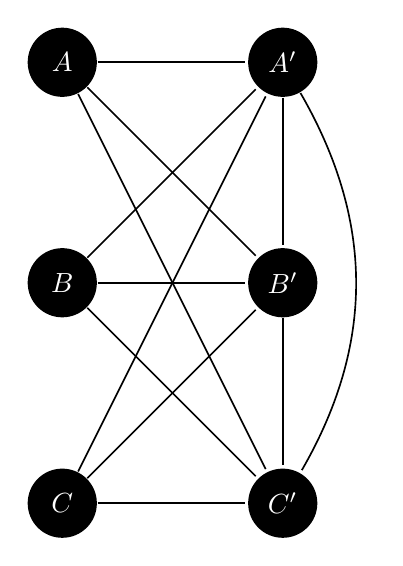
\begin{tikzpicture}[-,>=stealth',shorten >=1pt,auto,node distance=2.8cm,
                    semithick]
  \tikzstyle{every state}=[fill=black,draw=none,text=white]

  \node[state] (A)                    {$A$};
  \node[state]         (B) [below of=A] {$B$};
  \node[state]         (C) [below of=B] {$C$};
  \node[state]         (A1) [right  of=A] {$A'$};
  \node[state]         (B1) [right of=B] {$B'$};
  \node[state]         (C1) [right of=C] {$C'$};


  \path (A) edge        node {} (A1)
        (A) edge        node {} (B1)
        (A) edge        node {} (C1)
        (B) edge        node {} (A1)
        (B) edge        node {} (B1)
        (B) edge        node {} (C1)
        (C) edge        node {} (A1)
        (C) edge        node {} (B1)
        (C) edge        node {} (C1)
        (A1) edge        node {} (B1)
        (A1) edge [bend left] node {} (C1)
        (B1) edge        node {} (C1);
\end{tikzpicture}
$$

\subsection{Detecting Infections}
\label{infections}

To detect infections, we use Pointwise Mutual Information \cite{pmi} to identify salient bigrams in each site in each timestep. Whenever these occur multiple times across the entire dataset, they may be infections. We examine the occurences of each ngram to see if it appears in bursts, and if it does, we designate it an infection.


\subsection{Learning Parameters}


We used the method for finding the MLE estimate in triangulated graphs described in \cite{wainwright} to learn the weights of our edges. The model is trained on every pairs of steps $t,t+1$. We define indicator functions 
$$\I[s]=\begin{cases}1&$Infection occurs in site $s\\0& s $ is not uninfected$\end{cases}$$ 
and
$$\I[s,t;j,k]=\begin{cases}1&$if infection is present in site $s$ ($j=1$) and $t$ ($k=1$)$\\
0& $otherwise$\end{cases}$$ 
Parameters are the logs of the expectations of these indicator functions.\\


\subsection{Inference Problem}
Our question “Given a cascade at time $t$, what will be the state of the cascade at time $t+1$ can be restated as the following variational problem:\\
Given that we have learned our parameters $\theta_s$ and $\theta_st$, and that we have observed half of the nodes $X=\{x_1 ,x_2,\dots,x_n\}$ representing all of our sites at time $t$, what is the MLE assignment to the nodes $X^*=\{x^*_1 ,x^*_2,\dots,x^*_n\}$?\\
This optimization over $2^n$ possible assignments with $n$ equal to the number of sites under examination is NP-complete.\\
Good approximations are found by searching the parameter space. 

\section{Datasets}
\label{data}

Our algorithm is evaluated on three datasets.
\begin{description}
  \item[MemeTracker] A collection of popular newssites during the campaign season of 2008. Sites are blogs and major media sources. Memes detected via the Memetracker algorithm \cite{memetracker} are designated infections.
  \item[StackExchange] There are 28 different sites on StackExchange. Pointwise Mutual Information \cite{pmi} identifies salient bigrams. Common bigrams detected by PMI that occur in bursts are infections.
  \item[Synthetic] Infections are randomly initialized and spread through sampling via MCMC from generated parameters.
\end{description}
Our algorithm is evaluated on three datasets: a reddit dataset scraped from reddit.com, a stack-exchange dataset, and a synthetic dataset.

\subsection{Reddit}
Reddit is divided into thousands of \textit{subreddits}, each of which is targeted towards specialty interests. There is a many-to-many relationship between users and subreddits, with most users active in many subreddits and most subreddits populated with many users.

We looked at the top 20 subreddits in terms of popularity, and as these are so active, we set our timestep to be six hours. For each timestep, we formed a document of all of the post titles present during that time. A contagion was defined as described in \ref{infections}.


\subsection{StackExchange}

\subsection{Synthetic Dataset}


% Figure showing some structure of connections between reddits

% Figure showing some structure of connections between conferences

\section{Experiments}
\label{experiments}

We conducted three sets of experiements, on the \texttt{reddit} dataset, the \texttt{StackExchange} dataset, and the synthetic dataset. Each of these was similar, in that we used $n$-fold cross-validation to predict cascades with our algorithm, and with the edge weights learned by NetInf.

\section{Results}
\label{results}

% predicted prevalence of phrase based on network vs based on entire thing

% predicted network structure given phrases

\section{Discussion}
\label{discussion}


\bibliography{sources}{}
\label{refs}
\bibliographystyle{plain}

\end{document}